\documentclass[a4paper,12pt]{article}
\usepackage[utf8]{inputenc}
\usepackage[T1]{fontenc}
\usepackage[spanish]{babel}
\usepackage{amsmath,amssymb}
\usepackage{geometry}
\usepackage{graphicx}
\usepackage{float}

\geometry{margin=1in}

\title{Actividad sesi\'on 02}
\author{Juan Diego G\'omez Chavarro}
\date{22/02/2024}

\begin{document}
	
	\maketitle
	
	\section{Probabilidad frecuentista}
	
	\begin{itemize}
		\item Suponga que tienen dos dados balanceados de seis caras cada uno. ¿La probabilidad de obtener un uno en ambos dados será la misma si se lanzan simultáneamente o si se lanzan de manera consecutiva?
		\item En una baraja de 52 cartas, ¿cuál es la probabilidad de obtener un póker de ases en la primera mano?
		\item En una baraja de 52 cartas, ¿cuál es la probabilidad de recibir tres cartas cuya suma sea 21?
	\end{itemize}
	
	
	\subsection{Soluci\'on item 1}
	
	La probabilidad \( P(A \cap B) \) de obtener un uno en el primer dado (evento \( A \)) y obtener un uno en un segundo dado (evento \( B \)) no se ve afectada por el orden de lanzamiento de los dados, ya que los eventos \( A \) y \( B \) son independientes entre sí.
	
	Por lo tanto, \( P(A|B) \) y \( P(B|A) \) son iguales a las probabilidades individuales de cada evento, es decir, \( P(A) \) y \( P(B) \). En este orden de ideas:
	
	\[
	P(A \cap B) = P(A) \cdot P(B) = \frac{1}{6} \times \frac{1}{6} = \frac{1}{36}
	\]
	
	
	
	\subsection{Solución ítem 2}
	
	Una mano de póker estándar consiste en 5 cartas extraídas de una baraja de 52 cartas. El número total de formas en que se pueden seleccionar 5 cartas de 52 (sin importar el orden) es:
	
	\begin{equation}
		\text{Total de manos posibles} = \binom{52}{5} = \frac{52!}{5!(52-5)!} = 2,598,960
	\end{equation}
	Para obtener un póker de ases, necesitamos exactamente 4 ases y una carta adicional cualquiera.
	
	\begin{itemize}
		\item Hay 4 ases en la baraja y debemos elegir todos ellos:
		\begin{equation}
			\binom{4}{4} = 1
		\end{equation}
		\item La quinta carta puede ser cualquiera de las 48 cartas restantes (las que no son ases):
		\begin{equation}
			\binom{48}{1} = 48
		\end{equation}
	\end{itemize}
	
	Por lo tanto, el número de manos que contienen un póker de ases es:
	
	\begin{equation}
		\binom{4}{4} \times \binom{48}{1} = 1 \times 48 = 48
	\end{equation}
	
	
	La probabilidad de obtener un póker de ases es el número de casos favorables dividido entre el total de casos posibles:
	
	\begin{equation}
		P(\text{póker de ases}) = \frac{48}{2,598,960}
	\end{equation}
	
	Calculamos el valor numérico:
	
	\begin{equation}
		P(\text{póker de ases}) \approx 0.0000185
	\end{equation}
	
	Es decir, aproximadamente un 0.00185\% (menos de 2 manos en 100,000).
	
	
	
	
	
	\subsection{Soluci\'on item 3}
		
		Se muestra a continuación la demostración para calcular la probabilidad de recibir tres cartas cuya suma sea 21 en una baraja de 52 cartas.
		
		El n\'umero de formas de escoger 3 cartas (sin importar el orden) es:
			\[
			\binom{52}{3} = \frac{52!}{3!(52- 3)!} = 22100.
			\]
		Ahora se busca una tripleta (sin importar el orden) de tres cartas que al ser sumadas den 21:
		\begin{align*}
			&(10, 10, 1) \quad (10+10+1 = 21)\\[1mm]
			&(10, 9, 2) \quad (10+9+2 = 21)\\[1mm]
			&(10, 8, 3) \quad (10+8+3 = 21)\\[1mm]
			&(10, 7, 4) \quad (10+7+4 = 21)\\[1mm]
			&(10, 6, 5) \quad (10+6+5 = 21)\\[1mm]
			&(9, 9, 3) \quad (9+9+3 = 21)\\[1mm]
			&(9, 8, 4) \quad (9+8+4 = 21)\\[1mm]
			&(9, 7, 5) \quad (9+7+5 = 21)\\[1mm]
			&(9, 6, 6) \quad (9+6+6 = 21)\\[1mm]
			&(8, 8, 5) \quad (8+8+5 = 21)\\[1mm]
			&(8, 7, 6) \quad (8+7+6 = 21)\\[1mm]
			&(7, 7, 7) \quad (7+7+7 = 21)
		\end{align*}
		Se procede a calcular el numero de formas para cada combinaci\'on. teniendo en cuenta que hay cuatro cartas de cada una.

	
	\begin{enumerate}
		\item \textbf{$(10, 10, 1)$:}
		\begin{itemize}
			\item Elegir 2 cartas de valor 10: $\displaystyle \binom{16}{2} = \frac{16!}{2!(16-2)!} = 120$ formas.
			\item Elegir 1 as: $\displaystyle \binom{4}{1} = \frac{4!}{1!(4-1)!} = 4$ formas.
		\end{itemize}
		
		\[
		\text{Total: } 120 \times 4 = 480.
		\]
		\item \textbf{$(10, 9, 2)$:}
		\[
		\text{Total: } 16 \times 4 \times 4 = 256.
		\]
		
		\item \textbf{$(10, 8, 3)$:}
		\[
		\text{Total: } 16 \times 4 \times 4 = 256.
		\]
		
		\item \textbf{$(10, 7, 4)$:}
		\[
		\text{Total: } 16 \times 4 \times 4 = 256.
		\]
		
		\item \textbf{$(10, 6, 5)$:}
		\[
		\text{Total: } 16 \times 4 \times 4 = 256.
		\]
		
		\item \textbf{$(9, 9, 3)$:}
		\begin{itemize}
			\item Elegir 2 cartas de 9: $\displaystyle \binom{4}{2} = 6$ formas.
			\item Elegir 1 carta de 3: 4 formas.
		\end{itemize}
		\[
		\text{Total: } 6 \times 4 = 24.
		\]
		
		\item \textbf{$(9, 8, 4)$:}
		\[
		\text{Total: } 4 \times 4 \times 4 = 64.
		\]
		
		\item \textbf{$(9, 7, 5)$:}
		\[
		\text{Total: } 4 \times 4 \times 4 = 64.
		\]
		
		\item \textbf{$(9, 6, 6)$:}
		\begin{itemize}
			\item 9: 4 formas.
			\item Elegir 2 cartas de 6: $\displaystyle \binom{4}{2} = 6$ formas.
		\end{itemize}
		\[
		\text{Total: } 4 \times 6 = 24.
		\]
		
		\item \textbf{$(8, 8, 5)$:}
		\begin{itemize}
			\item Elegir 2 cartas de 8: $\displaystyle \binom{4}{2} = 6$ formas.
			\item Elegir 1 carta de 5: 4 formas.
		\end{itemize}
		\[
		\text{Total: } 6 \times 4 = 24.
		\]
		
		\item \textbf{$(8, 7, 6)$:}
		\[
		4 \times 4 \times 4 = 64.
		\]
		
		\item \textbf{$(7, 7, 7)$:}
		\[
		\binom{4}{3} = 4.
		\]
	\end{enumerate}
	
	En este orden de ideas, el numero total de formas de obtener estas combinaciones son:
	\[
	480 + 256 + 256 + 256 + 256 + 24 + 64 + 64 + 24 + 24 + 64 + 4 = 1772 \text{ Formas}.
	\]
	
	
	La probabilidad \(P\) de obtener tres cartas cuya suma sea 21 es:
	\[
	P = \frac{\text{Número de casos favorables}}{\text{Número total de casos}} = \frac{1772}{22100}.
	\]

	en conclusion la probabilidad de obtener tres cartas cuya suma sea 21 es:
	\[
	P \approx 0.0802 \quad (8.02\%).
	\]
	
	\section{Soluci\'on enunciado 2}
	
	\begin{itemize}
		\item La probabilidad de tener una enfermedad es del 1%.
		\item Si una persona TIENE la enfermedad, el test lo detecta el 95 \% de las veces.
		\item Si una persona esta sana, el test podría detectar la enfermedad un 5\% de las veces.
		\item Un paciente tomó el test y le dio positivo.  ¿Cuál es la probabilidad de que el paciente SI TENGA la enfermedad?
	\end{itemize}
	 Definimos las siguientes probabilidades:
	 
	 \[
	 P(\text{enfermo}) = 0.01
	 \]
	 
	 \[
	 P(\text{sano}) = 1 - P(\text{enfermo}) = 0.99
	 \]
	 
	 \[
	 P(\text{Test positivo} \mid \text{enfermo}) = 0.95
	 \]
	 
	 \[
	 P(\text{Test positivo} \mid \text{sano}) = 0.05
	 \]
	 
	 Queremos calcular:
	 
	 \[
	 P(\text{enfermo} \mid \text{Test positivo}) = \frac{P(\text{Test positivo} \mid \text{enfermo}) \cdot P(\text{enfermo})}{P(\text{Test positivo})}
	 \]
	 
	 Como no conocemos \( P(\text{Test positivo}) \), lo calculamos utilizando la ley de probabilidad total:
	 
	 \[
	 P(\text{Test positivo}) = P(\text{enfermo}) \cdot P(\text{Test positivo} \mid \text{enfermo}) + P(\text{sano}) \cdot P(\text{Test positivo} \mid \text{sano})
	 \]
	 
	 Sustituyendo los valores:
	 
	 \[
	 P(\text{Test positivo}) = (0.01 \times 0.95) + (0.99 \times 0.05)
	 \]
	 
	 \[
	 P(\text{Test positivo}) = 0.0095 + 0.0495 = 0.059
	 \]
	 
	 Ahora aplicamos el teorema de Bayes:
	 
	 \[
	 P(\text{enfermo} \mid \text{Test positivo}) = \frac{P(\text{Test positivo} \mid \text{enfermo}) \cdot P(\text{enfermo})}{P(\text{Test positivo})}
	 \]
	 
	 \[
	 P(\text{enfermo} \mid \text{Test positivo}) = \frac{0.95 \times 0.01}{0.059}
	 \]
	 
	 \[
	 P(\text{enfermo} \mid \text{Test positivo}) = \frac{0.0095}{0.059} = 0.161
	 \]
	
	
	
	\section{Soluci\'on enunciado 3}
	
	
	\begin{itemize}
		\item Obtenga un muestra de 100 datos de una distribución normal con media
		CERO y varianza UNO.  Para ello implemente la transformación de Box-Muller.
		\item Grafique el histograma de las muestras para verificar visualmente que son gausianas.
		\item Aplique el criterio de Kolmogorov-Smirnov a las muestras obtenidas para compararlas primero con una gausiana de referencia, y luego con una exponencial.
		\item Repita el proceso con una muestra de tan solo 10 datos. Concluya lo observado
	\end{itemize}
	
	
	
	
	\subsection{Soluci\'on}
	
	Para obtener una muestra de 100 y 10 datos de una distribuci\'on normal con media cero y varianza uno, se utiliz\'o la transformaci\'on de Box-Muller. Esta t\'ecnica genera pares de variables aleatorias independientes con distribuci\'on normal est\'andar a partir de dos variables aleatorias independientes con distribuci\'on uniforme en el intervalo $[0, 1]$.
	
	\begin{figure}[H]
		\centering
		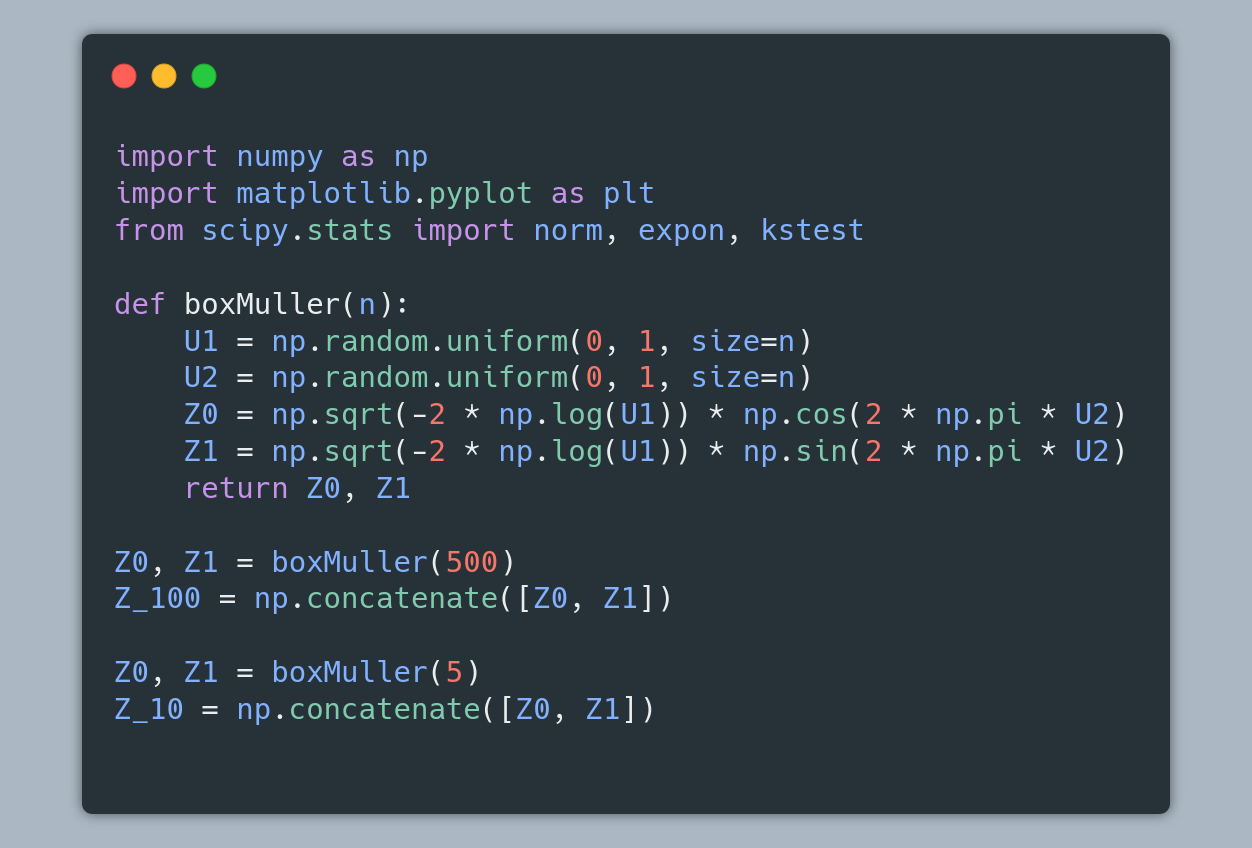
\includegraphics[width=0.8\textwidth]{carbon1.png}
		\caption{Muestras utilizando Box-muller}
		\label{fig:ejemplo}
	\end{figure}
	
	Para verificar la forma de la distribuci\'on de las muestras generadas, se construyeron histogramas para las muestras de 100 y 10 datos, respectivamente. Se observa que la distribuci\'on de 100 muestras tiene una forma cercana a la gaussiana, mientras que la de 10 muestras presenta mayor variabilidad y menor semejanza a la distribuci\'on esperada.
	
	\begin{figure}[H]
		\centering
		\begin{minipage}{0.45\textwidth}
			\centering
			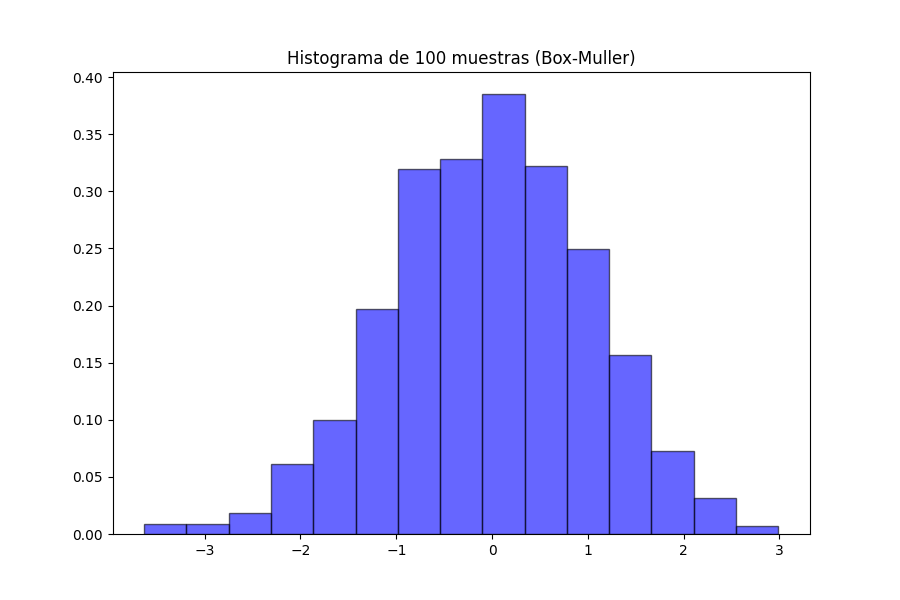
\includegraphics[width=\textwidth]{histograma100.png}
			\caption{Histograma de 100 muestras.}
			\label{fig:izquierda}
		\end{minipage}
		\hfill
		\begin{minipage}{0.45\textwidth}
			\centering
			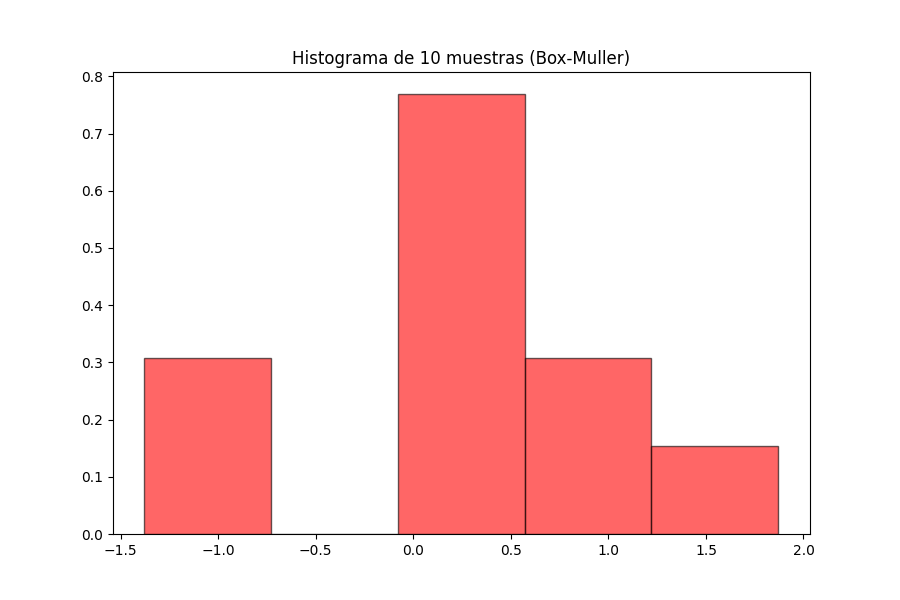
\includegraphics[width=\textwidth]{histograma10.png}
			\caption{Histograma de 10 muestras.}
			\label{fig:derecha}
		\end{minipage}
	\end{figure}
	
	

	Para evaluar cuantitativamente si las muestras generadas provienen de una distribuci\'on normal, se aplic'o la prueba de Kolmogorov-Smirnov. Se compararon las muestras tanto con una distribuci\'on normal de referencia como con una distribuci'on exponencial para verificar cu\'an bien se ajustan.
	
	\begin{figure}[H]
		\centering
		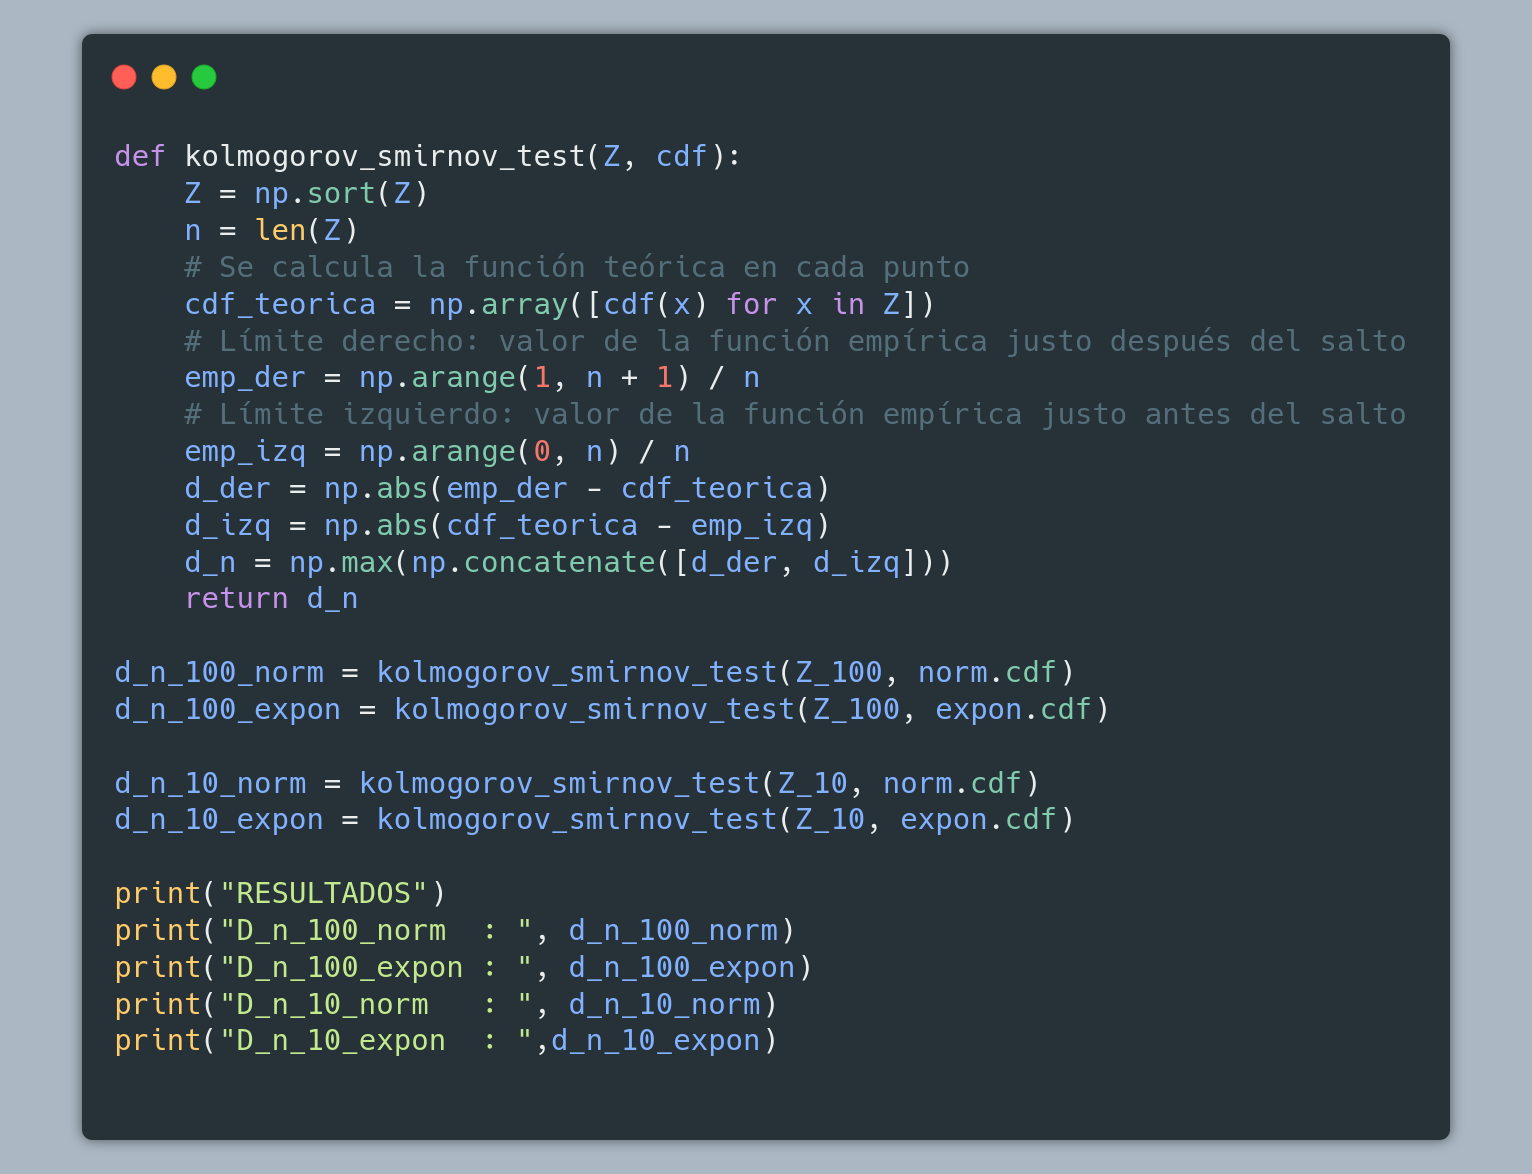
\includegraphics[width=0.8\textwidth]{carbon2.png}
		\caption{c\'alculo de Kolmogorov-Smirnov}
		\label{fig:ejemplo}
	\end{figure}
	
	Los resultados obtenidos se presentan a continuaci\'on:
	
	\begin{figure}[H]
		\centering
		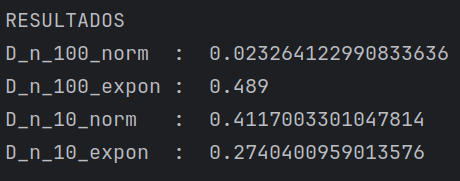
\includegraphics[width=0.4\textwidth]{resultados.png}
		\caption{Resultados KS}
		\label{fig:ejemplo}
	\end{figure}
	
	Para la muestra de 100 datos, los resultados de la prueba de Kolmogorov-Smirnov muestran que los valores generados se ajustan bien a una distribución normal, mientras que para la muestra de 10 datos la diferencia es mayor. Esto se debe a que, con menos datos, hay más variabilidad y es más difícil determinar con precisión la distribución real. Esto muestra que usar muestras más grandes ayuda a obtener resultados más confiables en este tipo de pruebas.
	
\end{document}
